\documentclass[a4paper,12pt]{jarticle}
\input ./chap01_preamble.tex
\graphicspath{%
  {../text01-img/}%
}
% !TEX root = ./chap01_02.tex
\begin{document}
\section{ラズベリーパイになれよう(1)}
\subsection{ファイル、フォルダ}
\ \ コンピュータやラズベリーパイの中にあるデータ(音楽、動画、写真、テキストなど)はすべてファイルとして扱われています。しばしばファイルには.(ドット)から始まる「拡張子」がついており、ファイルがどんな種類なのかを表します。例えば画像の場合は.jpgや動画ファイルの場合はmp4、テキストファイルは.txt、ホームページの場合は.htmlがついています。

ファイルの他にフォルダというものがあります。フォルダはファイルをまとめたものです。ファイルを書類としてフォルダはバインダと考えるとわかりやすいでしょう。フォルダのなかにフォルダをいれることもできます。



\begin{figure}[hb]
  \centering
  \begin{minipage}{13.148cm}


    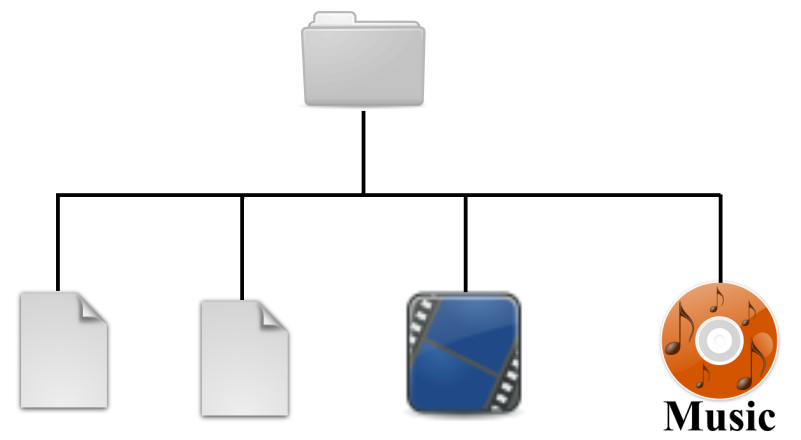
\includegraphics[width=13.148cm]{figure15.png}
    {\upshape
      \newline
      Figure \stepcounter{Figure}{\theFigure}:
      フォルダ、ファイルの関係}
  \end{minipage}
\end{figure}

\begin{minipage}{\textwidth}
  \begin{minipage}{5.562cm}
    \centering
    \textbf{(左)クリック}
    \flushleft

    カチッ\\
    \centering
    \raisebox{20mm}{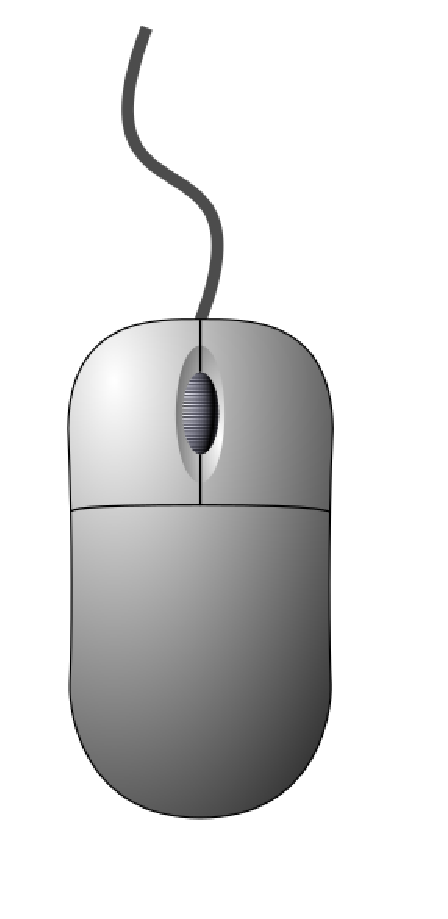
\includegraphics[width=1.651cm,height=3.53cm]{textbook-img076.eps}}

    \flushleft
    マウスの左側を一度押すこと、アプリなど開きたいときに使おう
  \end{minipage}
  \begin{minipage}{5.562cm}
    \centering
    \textbf{ダブルクリック}
    \flushleft

    カチカチッ\\
    \centering
    \raisebox{20mm}{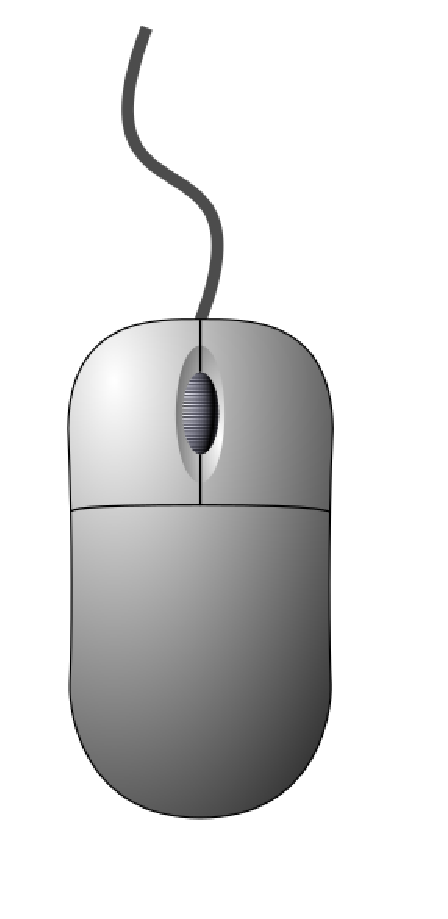
\includegraphics[width=1.651cm,height=3.53cm]{textbook-img076.eps}}


    \flushleft
    マウスの左側を二回続けて押すこと。 デスクトップのフォルダなどを開くときに使うよ
  \end{minipage}
  \begin{minipage}{5.562cm}
    \centering
    \textbf{~~~~~右クリック}
    \flushleft

    \hspace{3cm} カチッ\\
    \centering
    \raisebox{20mm}{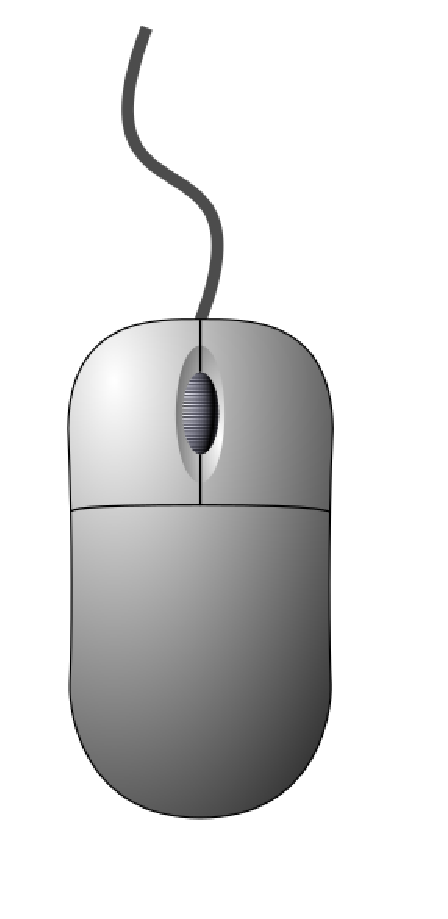
\includegraphics[width=1.651cm,height=3.53cm]{textbook-img076.eps}}


    \flushleft
    マウスの右側を一度押すこと。メニューなどを表示したいときに使うよ
  \end{minipage}
\end{minipage}


\clearpage

\refstepcounter{Exercise}
\subsection{\theExercise 自分のフォルダを確認しよう}
まず、みなさんがこの授業で使う「自分のフォルダ」を確認しましょう。
このとき、注意してもらいたいことが1つあります。
さきほど、みなさんには「ユーザ名」と「パスワード」を設定してもらいました。
そのとき設定した「ユーザ名」によって、みなさんひとりひとりの「自分のフォルダ」の名前が変わります。
どこが変わるのか、じっさいに見てみましょう。\\

{\bf \large 考え方}\\
\begin{figure}[ht]
\begin{minipage}{\textwidth}
  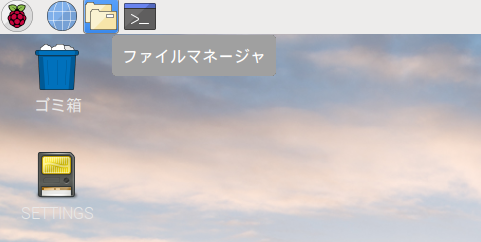
\includegraphics[width=6.472cm]{textbook-img032.png}
  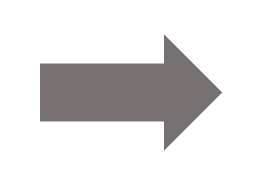
\includegraphics[width=2.094cm]{textbook-img035.png}
  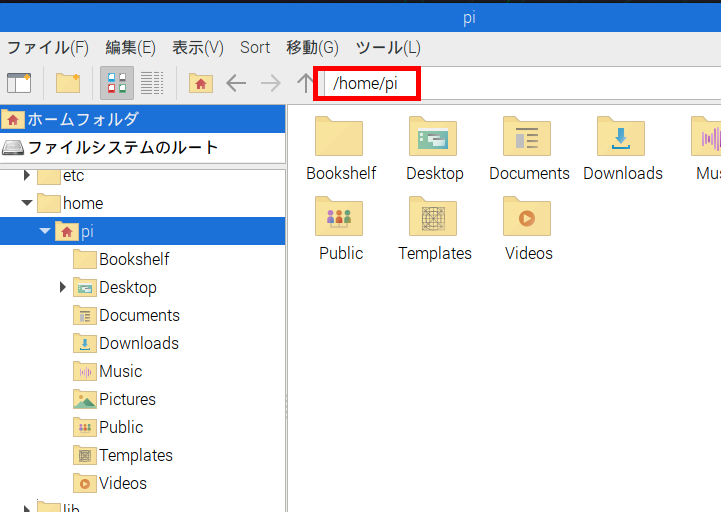
\includegraphics[width=8.301cm]{textbook-img1020.png}
\end{minipage}
\begin{minipage}{0.4\textwidth}
  1
  ディスプレイの左上の、黄色いアイコンをクリック
\end{minipage}
\vspace{20pt}
\hfill
\begin{minipage}{0.4\textwidth}
  2
  上の図のように、ファイルマネージャーが開いて、自分のフォルダが表示されます。(ウィンドウの色が違うかもしれませんが、色はあとで変えられます)
\end{minipage}
\end{figure}
\\ファイルマネージャーは、初回起動時は自分のフォルダを表示します。
この、ファイルマネージャの写真の赤枠で囲ったところには、自分のフォルダのパスが書いてあります。
パスについての詳しい説明は、以降の回で出てくるので、今はとりあえずフォルダ、ファイルの「住所」と考えてください。
この画像では、/home/piと書いてあります。ですが、みなさんは違うはずです。
\textbf{\color{red}ここに、さいしょに設定した「ユーザ名」が反映されます。}
たとえば、「takeshi」というユーザ名を設定した場合、この赤枠の中は、
/home/takeshiになります。
\vspace{20pt}

\refstepcounter{Question}\theQuestion\\
自分のフォルダのパス(右上の画像の赤い枠で囲まれた部分)を、下の空欄に書き写してみよう
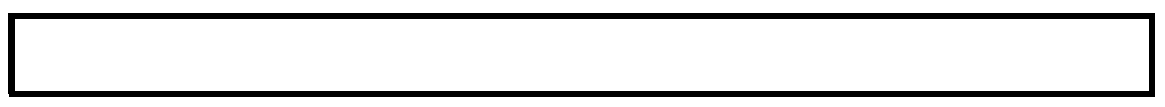
\includegraphics[width=17cm]{textbook-img1021.png}
\clearpage

\refstepcounter{Exercise}
\subsection{\theExercise フォルダを作成しよう}
Documentsフォルダ直下にtaro、hanako、saburoという名前のフォルダを作成しましょう。\\

{\bf \large 考え方}
\begin{figure}[ht]
  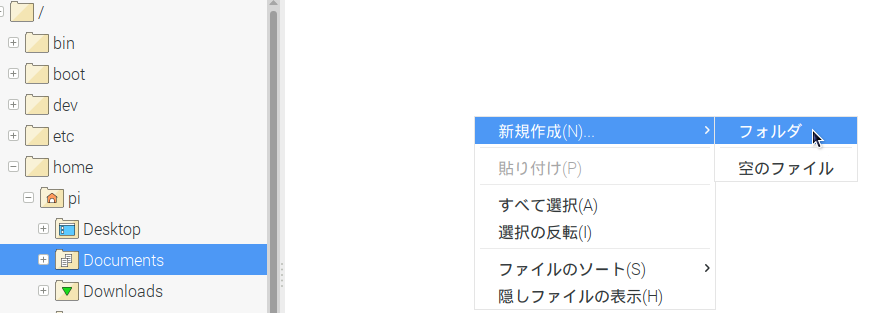
\includegraphics[width=0.9\textwidth]{textbook-img034.png}
    \centering
    \\1
    ファイルマネージャーの空白部分で右クリックし 「New Folder」にカーソルを合わせてクリック
    \vspace{60pt}
  \begin{minipage}{\textwidth}
    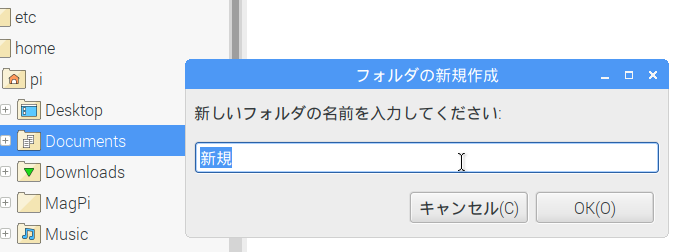
\includegraphics[width=0.9\textwidth]{textbook-img036.png}
  \end{minipage}
    2
    フォルダ名の入力を求められるので、付けたい名前を入力しよう
\end{figure}
\clearpage
{\bf\large 考え方(続き)}
\begin{figure}[hb]
  \centering
  %[Warning: Image ignored] % Unhandled or unsupported graphics:
  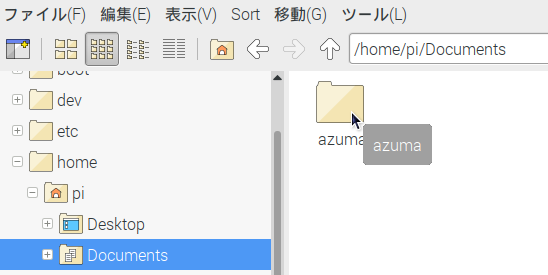
\includegraphics[width=11.398cm]{textbook-img038.png}
  \centering
  \begin{minipage}{13.001cm}
    3
    名前を入力し、OKを押すと上の画像のようにフォルダが作成されます
  \end{minipage}

\end{figure}
\begin{figure}[hb]
  \centering
  \begin{minipage}{0.8\textwidth}
    {	\large
      フォルダは大事です。

      フォルダに、画像やプログラムのコードを保存しておくので、わかりやすく関係性のある名前を付けてあげましょう

      \bigskip
      ファイルやフォルダの名前は、
      空白の入らない半角ローマ字にしておくと、
      後でプログラムから使う時に便利だよ
    }
  \end{minipage}
\end{figure}
\clearpage
\begin{figure}[ht]
  \flushleft{\bf\large 答え}
  \vspace{8mm}\\
  \centering
  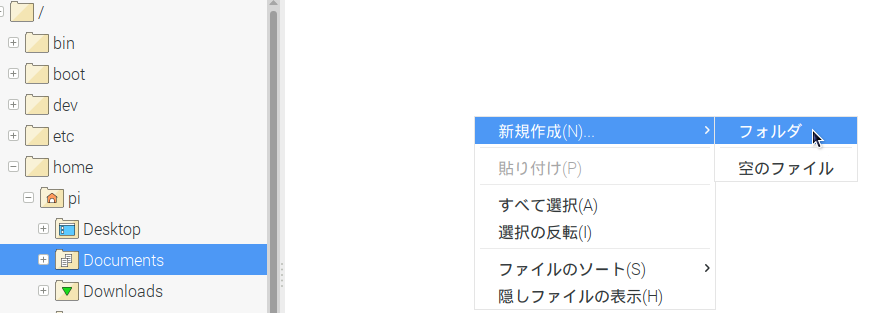
\includegraphics[width=13.33cm]{textbook-img034.png}
  \begin{minipage}{\textwidth}
    1
    左上のフォルダアイコンをクリックし

    フォルダマネージャー上で右クリックし、上の画像のようにしよう
  \end{minipage}

  \centering
  %[Warning: Image ignored] % Unhandled or unsupported graphics:
  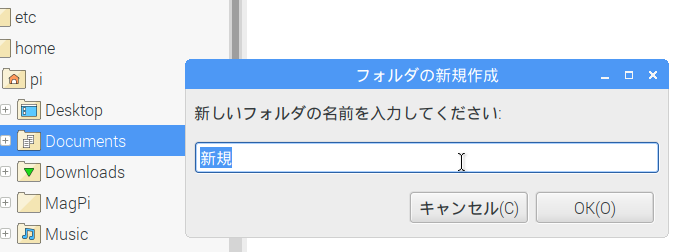
\includegraphics[width=12.483cm]{textbook-img036.png}
  \begin{minipage}{\textwidth}
    2
    \ 「New Folder」を選び、名前設定に行こう
  \end{minipage}

  \centering
  %[Warning: Image ignored] % Unhandled or unsupported graphics:
  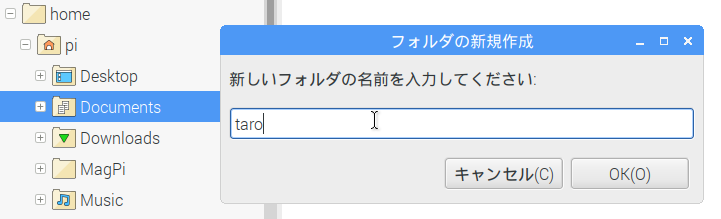
\includegraphics[width=12.776cm]{textbook-img039.png}
  \begin{minipage}{\textwidth}
    3 taroと名前を入力し、OKを押す
  \end{minipage}

  \centering
  %[Warning: Image ignored] % Unhandled or unsupported graphics:
  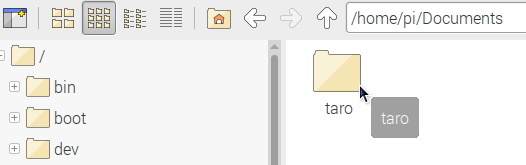
\includegraphics[width=12.659cm]{textbook-img040.png}
  \begin{minipage}{\textwidth}
    4 taroというフォルダを作成できていることを確認しよう
  \end{minipage}

\end{figure}
\clearpage
\begin{figure}
  \flushleft{\bf\large
    答え(続き)}\\
  \vspace{10mm}
  \centering
  %[Warning: Image ignored] % Unhandled or unsupported graphics:
  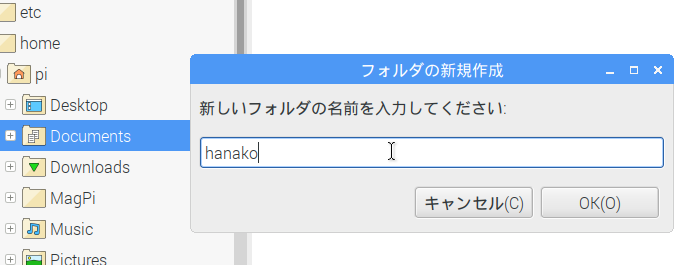
\includegraphics[width=14.289cm]{textbook-img041.png}
  \begin{minipage}{\textwidth}
    \ 5
    \ 先ほどと同じように右クリックから「New Folder」を選び、hanakoという名前でフォルダを作成
  \end{minipage}

  \centering
  %[Warning: Image ignored] % Unhandled or unsupported graphics:
  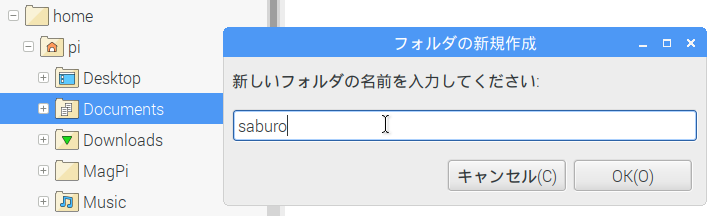
\includegraphics[width=13.884cm]{textbook-img042.png}
  \begin{minipage}{\textwidth}
    \ 6
    \ saburoというフォルダを先ほどと同じ方法で作成
  \end{minipage}

  \centering
  %[Warning: Image ignored] % Unhandled or unsupported graphics:
  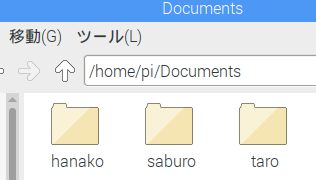
\includegraphics[width=8.359cm]{textbook-img043.png}
  \begin{minipage}{\textwidth}
    \ 7 \ taro , hanako ,
    saburoのフォルダが作成されていることを確認してみよう
  \end{minipage}
  \vspace{10mm}
  \flushleft
  \refstepcounter{Question}\theQuestion\label{Q:hasAnswer02-1}

  例題と同じ方法で、akahoshi、imaoka、hamanakaという名前のフォルダを作ろう

\end{figure}
\clearpage
\refstepcounter{Exercise}
\subsection{\theExercise フォルダを移動しよう}
Desktop直下に「space1」と「space2」を作り、「space1」の中に「move」フォルダを作り、「move」フォルダを「space2」に移動しよう

\flushleft{\bf\large 考え方}


\begin{figure}[ht]
  \centering
  %[Warning: Image ignored] % Unhandled or unsupported graphics:
  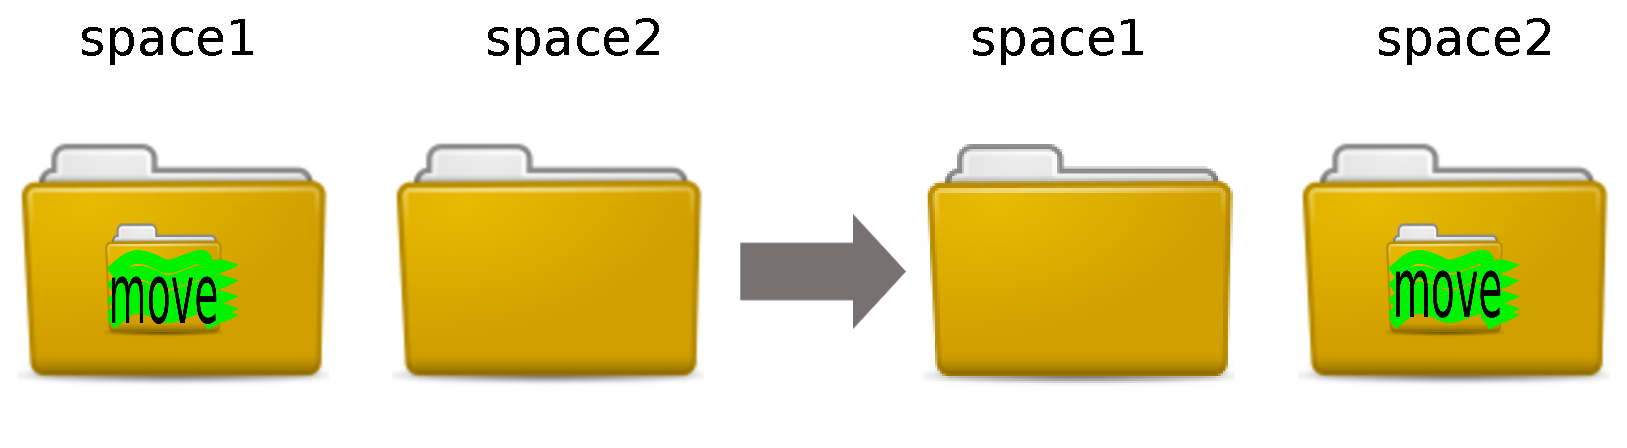
\includegraphics[width=0.8\textwidth]{fig15-1.eps}
  \begin{minipage}{15.297cm}
    フォルダやファイルは後からでも動かすことができるよ。
  \end{minipage}

  \begin{minipage}{5.963cm}
    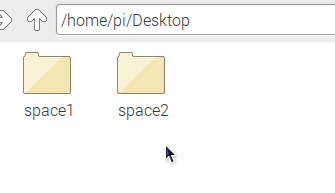
\includegraphics[width=3.604cm]{textbook-img051.png}
    {\flushleft
      1
      左側のDesktopをクリック しspace1とspace2を作成
    }
  \end{minipage}
  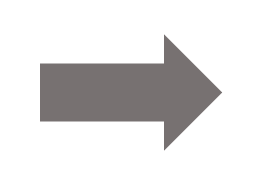
\includegraphics[width=2.168cm]{textbook-img052.png}
  \begin{minipage}{7.473cm}
    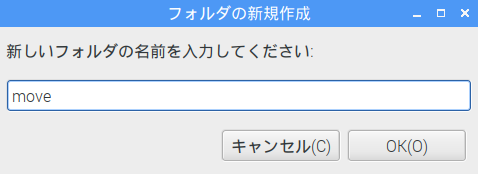
\includegraphics[width=5.166cm]{textbook-img050.png}
    {\flushleft
      2 space1の中にmoveフォルダを作成
    }
  \end{minipage}

  \centering
  \begin{minipage}{6.589cm}
    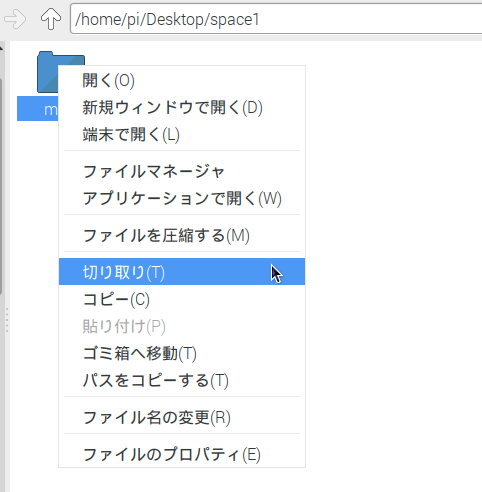
\includegraphics[width=3.584cm]{textbook-img048.png}
    {\flushleft
      3
      moveフォルダ上で右クリックし、 切り取りをクリック
    }
  \end{minipage}
  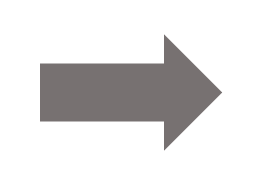
\includegraphics[width=2.168cm]{textbook-img049.png}
  \begin{minipage}{6.589cm}
    %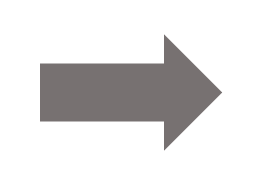
\includegraphics[width=2.168cm,height=1.542cm]{textbook-img047.png}
    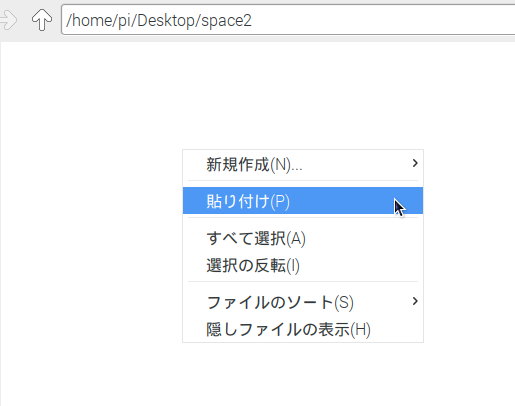
\includegraphics[width=5.225cm]{textbook-img046.png}
    {\flushleft
      4
      space2の中で右クリック、貼り付けをクリック
    }
  \end{minipage}

  %[Warning: Image ignored] % Unhandled or unsupported graphics:
  \begin{minipage}{6.589cm}
    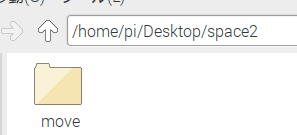
\includegraphics[width=7.218cm]{textbook-img045.png}
    {\flushleft
      5
      space1の中にあったmoveフォルダがspace2に移動しました
    }
  \end{minipage}


\end{figure}


\refstepcounter{Question}\theQuestion\label{Q:hasAnswer02-2}
「space1」フォルダ内に「rasp」フォルダを作り、さらにそのフォルダ内に「berry」フォルダを作成して「rasp」フォルダを「space2」フォルダに移動させよう。そして中身を確認しよう



\clearpage
\refstepcounter{Exercise}
\subsection{\theExercise ファイル名を変更しよう}
「before」という名前のフォルダをDocuments直下に1つ作り、その作成した後でフォルダ名を「after」に変えよう

\begin{figure}[ht]
  \flushleft{\bf\large 考え方}

  \centering
  %[Warning: Image ignored] % Unhandled or unsupported graphics:
  \begin{minipage}{1.978cm}
    
\includegraphics[width=1.5cm]{textbook-img044.png}
    frog
  \end{minipage}
  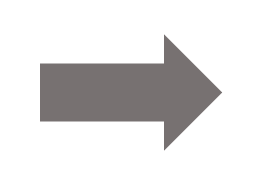
\includegraphics[width=2.168cm]{textbook-img052.png}
  \begin{minipage}{1.978cm}
    
\includegraphics[width=1.5cm]{textbook-img044.png}
    dog
  \end{minipage}
  \begin{minipage}{6.319cm}
    まちがったフォルダ名をつけたとき、名前を変えたいときなど
    に使います。
  \end{minipage}

  \begin{minipage}{6.656cm}
    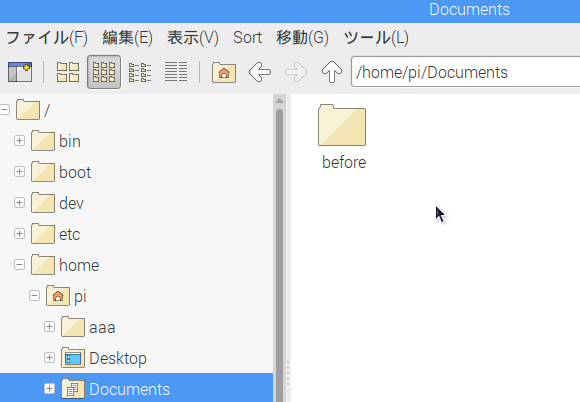
\includegraphics[width=6.96cm]{textbook-img058.png}
    \flushleft
    1
    左側のDocumentsをクリックし「before」フォルダを作成
  \end{minipage}
  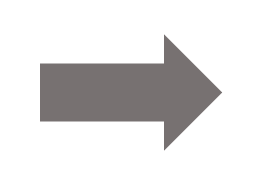
\includegraphics[width=2.168cm]{textbook-img052.png}
  \begin{minipage}{5.751cm}
    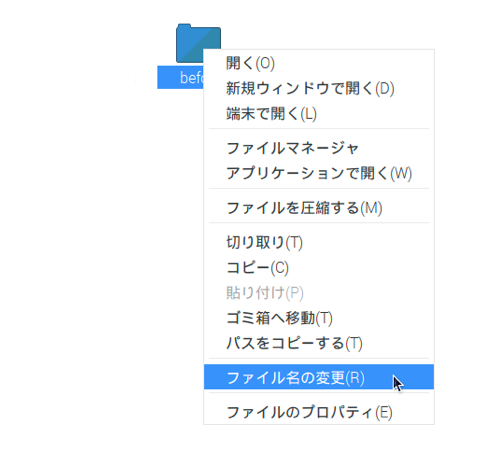
\includegraphics[width=6.555cm]{textbook-img057.png}
    \flushleft
    2 フォルダ上で右クリックし、

    ファイル名の変更をクリック
  \end{minipage}
  %[Warning: Image ignored] % Unhandled or unsupported graphics:

  \begin{minipage}{6.973cm}
    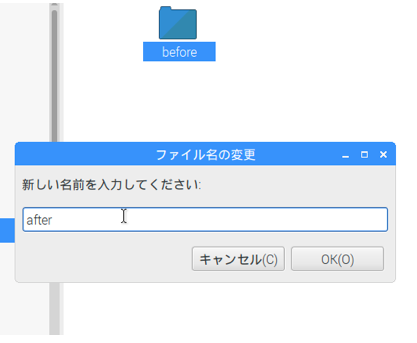
\includegraphics[width=6.973cm]{textbook-img055.png}
    3 名前を「after」に変更

    OKをクリック
  \end{minipage}
  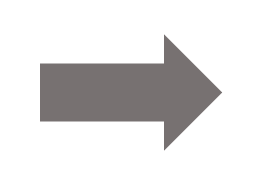
\includegraphics[width=1.919cm]{textbook-img053.png}
  \begin{minipage}{5.751cm}
    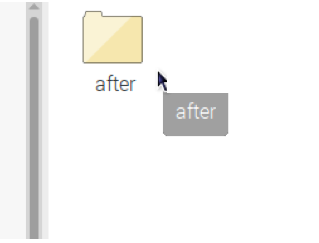
\includegraphics[width=5.92cm]{textbook-img056.png}
    4 変更を確認
  \end{minipage}
  \centering

  \begin{minipage}{5.751cm}
    フォルダ名の変更は、よく使うので覚えておこう
  \end{minipage}
\end{figure}


\refstepcounter{Question}\theQuestion\label{Q:hasAnswer02-3}

「miss\_name」という名前のフォルダを1つ作り、その作成した後でフォルダ名を「success\_name」に変えよう

\clearpage
\begin{figure}[ht]
  \refstepcounter{Exercise}
  \subsection{\theExercise 日本語入力と英字入力について}
  \ Text
  Editorを開き、アルファベットをa〜zまで入力しよう。その後「こんにちは」「こんばんは」「ごきげんよう」「さようなら」「ありがとう」をそれぞれ一行に入力しましょう。

  {\bf\large 考え方}


  \centering
  \begin{minipage}{\textwidth}
    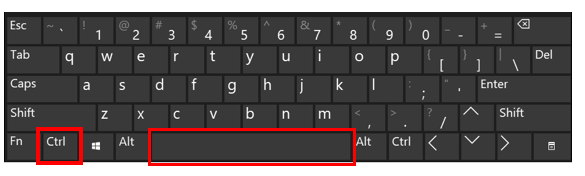
\includegraphics[width=7.459cm,height=2.245cm]{textbook-img065.png}
    \raisebox{10mm}
    {
      \begin{minipage}{0.5\textwidth}
        赤わくで囲んだ
        Ctrlとスペースを
        同時に押すことで
        英字入力と日本語入力を
        切り替えることができるよ
      \end{minipage}
    }
  \end{minipage}

  \begin{minipage}{6.984cm}
    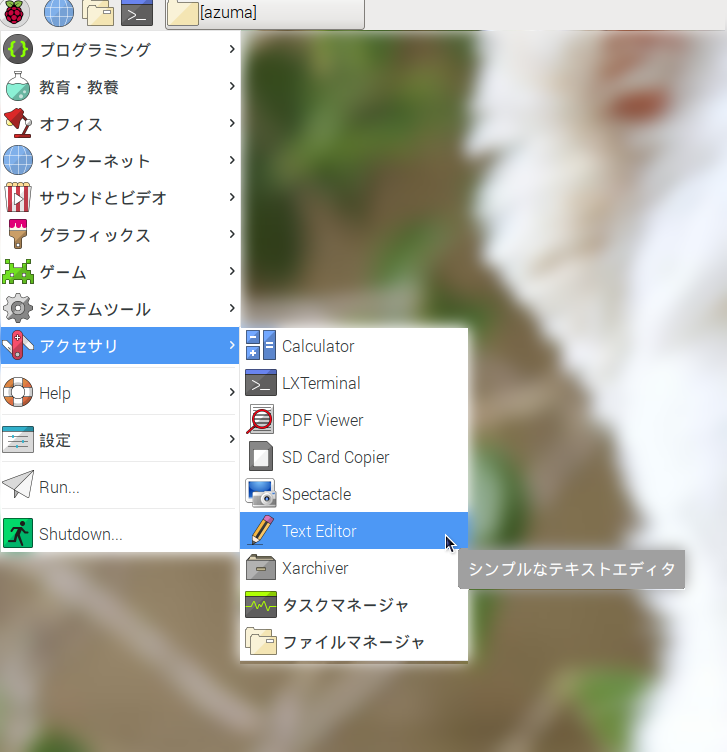
\includegraphics[width=5.408cm]{textbook-img064.png}
    \flushleft
    1
    ラズベリーのアイコンをクリックしてアクセサリー>Text
    editorを開こう
  \end{minipage}
  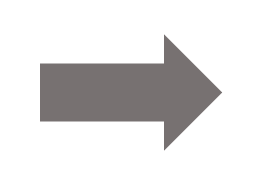
\includegraphics[width=1.919cm]{textbook-img053.png}
  \begin{minipage}{7.347cm}
    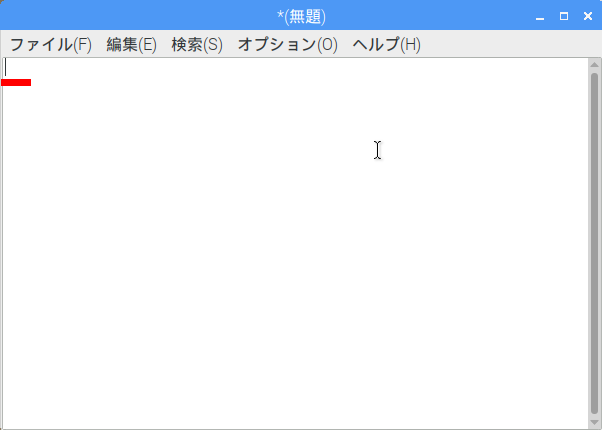
\includegraphics[width=7.897cm]{textbook-img063.png}
    \flushleft
    2.
    赤線が引かれているところをクリックしてテキストエディタにカーソル(縦棒)が入っていることを確認してください。
  \end{minipage}

  \begin{minipage}{7.238cm}
    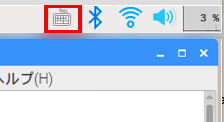
\includegraphics[width=6.643cm]{textbook-img059.png}
    \flushleft
    3. Ctrlとスペースキーを同時に押して

    英字入力に切り替えよう。アイコンがキーボードであることを確認しよう。
  \end{minipage}
  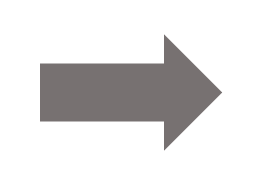
\includegraphics[width=1.919cm]{textbook-img053.png}
  \begin{minipage}{7.351cm}
    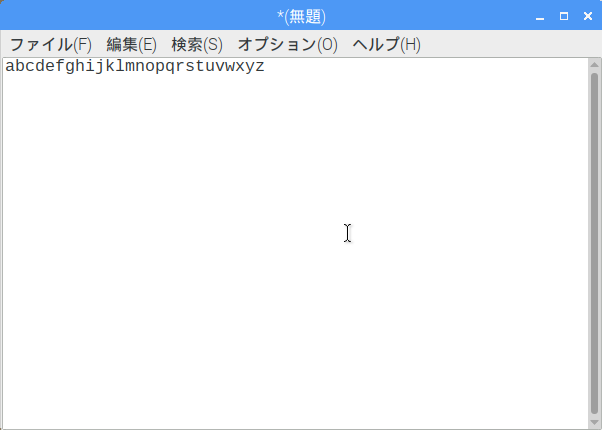
\includegraphics[width=6.514cm]{textbook-img061.png}
    \flushleft
    4. 英字入力でa〜zまで入力しよう
  \end{minipage}

  \begin{minipage}{6.73cm}
    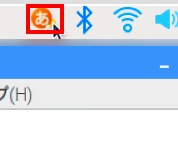
\includegraphics[width=4.029cm]{textbook-img062.png}
    \flushleft
    5. Ctrlとスペースキーを同時に押して
    アイコンが“あ”になったか確認しましょう。
  \end{minipage}
  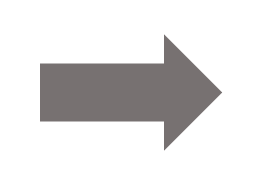
\includegraphics[width=1.919cm]{textbook-img053.png}
  \begin{minipage}{6.589cm}
    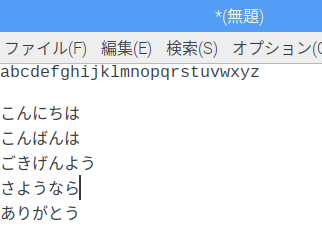
\includegraphics[width=4.914cm]{textbook-img060.png}
    \flushleft
    6. こんにちは〜ありがとうを入力\\
    7. 完成
  \end{minipage}



  \flushleft
  \refstepcounter{Question}\theQuestion\label{Q:hasAnswer02-4}
  Text editorでA〜Zを入力しよう

  ヒント

  英字入力時にshiftキーを押しながらアルファベットキーを打つと大文字で入力できます
\end{figure}
\clearpage
\begin{figure}[ht]
  \refstepcounter{Exercise}
  \subsection{\theExercise 半角入力と全角入力について}
  Text
  Editorを開き、半角入力でアルファベットをa〜zまで入力し、その後、全角入力で

  アルファベットa〜zまで入力しよう。全角と半角文字の違いを理解しよう。

  {\bf\large 考え方}

  \centering
  %[Warning: Image ignored] % Unhandled or unsupported graphics:
  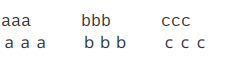
\includegraphics[width=5.978cm]{textbook-img066.png}
  \raisebox{8mm}{
    \begin{minipage}{6.762cm}
      {文字が小さいのが半角}\\
      {文字が大きいのが全角}
    \end{minipage}
  }

  \begin{minipage}{16.578cm}

    \bigskip

    アルファベットのサイズからも分かる通り、大きいサイズが全角で、小さいサイズが半角だと覚えておくといいよ
  \end{minipage}
  %[Warning: Image ignored] % Unhandled or unsupported graphics:
  \begin{minipage}{5.578cm}
    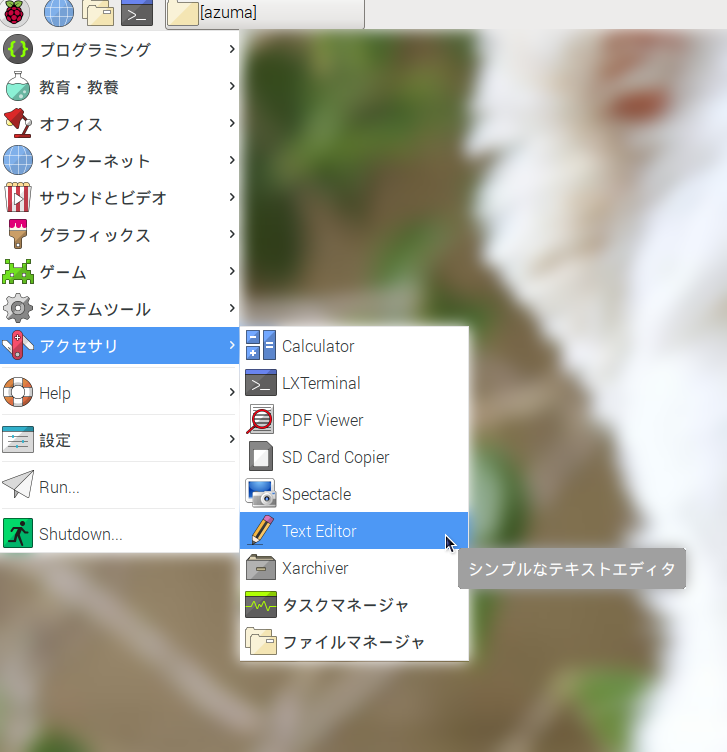
\includegraphics[width=5.172cm]{textbook-img067.png}
    \flushleft
    1 Text editorを開こう
  \end{minipage}
  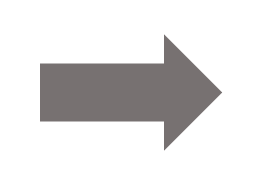
\includegraphics[width=1.919cm]{textbook-img053.png}
  \begin{minipage}{7.931cm}
    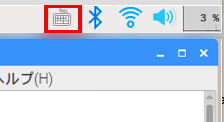
\includegraphics[width=7.868cm]{textbook-img059.png}
    \flushleft
    2
    キーボードのアイコンになっていることを確認して半角を入力しよう
  \end{minipage}
  \begin{minipage}{6.345cm}
    \includegraphics[width=4.889cm]{textbook-img059.png}
    \flushleft
    3
    半角のアルファベットを入力し終えたら右上のキーボードアイコンをクリック
  \end{minipage}
  \includegraphics[width=1.919cm]{textbook-img053.png}
  \begin{minipage}{7.524cm}
    \includegraphics[width=5.471cm]{textbook-img062.png}
    \flushleft
    4
    アイコンが変わったことを確認しよう
  \end{minipage}

  \begin{minipage}{7.173cm}
    \includegraphics[width=5.889cm]{textbook-img069.png}
    \flushleft
    5 アイコンを右クリックして、

    全角英数を選択
  \end{minipage}
  \includegraphics[width=1.919cm]{textbook-img053.png}
  \begin{minipage}{7.178cm}
    \includegraphics[width=7.471cm]{textbook-img070.png}
    \flushleft
    6 入力
  \end{minipage}

  \vspace{3mm}
  \begin{minipage}{16.578cm}
    {\centering\large
      プログラミングでアルファベット,記号を入力するときは
      半角(小さい文字)で入力しましょう
    }
  \end{minipage}

  \flushleft
  \refstepcounter{Question}\theQuestion\label{Q:hasAnswer02-5}

  Text editorで半角A〜Zと全角A〜Zを入力しよう

  ヒント


  英字入力時にshiftキーを押しながらアルファベットキーを打つと大文字で入力できます
\end{figure}
\clearpage
\begin{figure}[t]
  \subsection{ブラウザでけんさくをしよう}
  ブラウザを開いてけんさくをしよう。ブラウザを使用するとウェブサイトを開くことができます。もし、困ったことがあったら自分でけんさくをできるように使い方を覚えておきましょう。

  \refstepcounter{Exercise}
  \subsection{\theExercise 
    ブラウザ立ち上げとマウスそうさについて}
  ブラウザを立ち上げ、好きなものを調べよう

  {\bf\large 考え方}

  \begin{minipage}{\textwidth}
    \begin{minipage}{6.204cm}
      \includegraphics[width=5.426cm]{textbook-img071.png}
      1,デスクトップの左上のアイコンを左クリック
    \end{minipage}
    \includegraphics[width=1.505cm]{textbook-img073.png}
    \begin{minipage}{8.233cm}
      \includegraphics[width=8.373cm]{textbook-img075.png}
      2,
      ブラウザが立ち上がり、赤で囲われている部分を左クリック
    \end{minipage}
  \end{minipage}

  \hfill\begin{minipage}{7.78cm}
    {\centering
      \includegraphics[width=1.707cm]{textbook-img074.png}
    }\\
    \includegraphics[width=7.742cm]{textbook-img072.png}
    3,
    キーボードでけんさくしたいワード を入力しよう。入力し終えたらenterキーを押そう
  \end{minipage}

  \vspace{70mm}

\end{figure}
\clearpage
\begin{figure}
  Figure~\ref{seq:refFigure15}のように赤い四角で囲われているところにけんさくしたい言葉を入れてエンターキーを押すとけんさくができます。例えば”ねこ”とけんさくしてみましょう。
  \centering
  {\upshape
    \includegraphics[width=0.45\textwidth]{textbook-img077.png}

    Figure{\refstepcounter{Figure}\theFigure\label{seq:refFigure15}}: けんさくバー}


  \flushleft
  けんさくするとFigure~\ref{seq:refFigure16}このような感じになります。青線で囲んであるところは今けんさくした言葉です。赤線で囲われている\textbf{画像}をクリックすると画像をけんさくできます。クリックしてみましょう。


  \centering
  {\upshape
    \includegraphics[width=0.45\textwidth]{textbook-img078.png}
    \newline
    Figure {\refstepcounter{Figure}\theFigure\label{seq:refFigure16}}:
    ”ねこ”けんさく結果\\
    けんりの関けいで画像をぼかしてあります}

  \flushleft
  Figure~\ref{seq:refFigure17}のように”ねこ”の画像がたくさんでてきました。けんさくしたい言葉のけんさく結果を画像できました。\textbf{Web}をクリックすると先ほどのFigure~\ref{seq:refFigure16}のようなホームページけんさくに戻れます。


  \centering
  \upshape
    \includegraphics[width=0.45\textwidth]{textbook-img079.png}
    \newline
    Figure {\refstepcounter{Figure}\theFigure\label{seq:refFigure17}}:
    ”ねこ”画像けんさく結果

  \flushleft
  \refstepcounter{Question}\theQuestion

  \ \ 自分の好きなキーワードをけんさくしてみよう

\end{figure}
\clearpage
\begin{figure}[t]
  \refstepcounter{Exercise}
  \subsection{\theExercise キーボード入力の練習をしよう}
  \addtocounter{Exercise}{-1}\refstepcounter{Exercise}\label{E:typing}
  ブラウザで”
  Etyping”とけんさくし、キーボードタイピングサイトでタイピングに慣れよう

  \textbf{考え方}

  \textbf{タイピング}\ \ ・・・キーボードで文字を入力すること\ \
  \begin{minipage}{\textwidth}
    \raisebox{30mm}{		\begin{minipage}{0.65\textwidth}
        パソコンでの文字入力はローマ字入力が基本です。
        けんさくなどをしたいとき、キーボードで文字を入力します。
        今回はタイピング練習サイト”Etyping”でタイピングを
        練習しましょう。

        \includegraphics[width=8.087cm]{textbook-img081.png}
        \includegraphics[width=2.546cm]{textbook-img082.png}
      \end{minipage} }
    \includegraphics[width=4.928cm]{textbook-img080.png}
  \end{minipage}

  \centering


  {\centering
    \textbf{まずはタイピングゲームを開こう}
    \par}

  \centering

  \begin{minipage}{5.695cm}
    \includegraphics[width=5.523cm]{textbook-img071.png}
    1 左上のアイコンをクリックしよう
  \end{minipage}
  \includegraphics[width=2.094cm]{textbook-img084.png}
  \begin{minipage}{6.582cm}
    \includegraphics[width=6.985cm]{textbook-img083.png}
    2 けんさくらんに”Etyping”と入力しenterを押そう
  \end{minipage}


  \begin{minipage}{6.582cm}
    \includegraphics[width=6.796cm]{textbook-img086.png}
    3 サイトに入りましょう。赤わくで囲われているところのうち、一番上の「インターネットでタイピング練習 イータイピング」をクリックします。
  \end{minipage}
  \begin{minipage}{8.482cm}
    \includegraphics[width=8.714cm]{textbook-img085.png}
    赤線で線が引かれているところ、黒い四角で囲んであるアイコンをよく確かめてください。
  \end{minipage}






  \centering



\end{figure}
\clearpage

\begin{figure}
  \textbf{考え方(続き)}



  \centering

  \includegraphics[width=12.294cm,height=8.091cm]{textbook-img087.png}


  \begin{minipage}{4.252cm}
    4 ホームページが開けたら
    黒で囲んである

    \textbf{今すぐチェック!}

    をクリックしよう

  \end{minipage}
\end{figure}





\begin{figure}
  \centering
  \includegraphics[width=12.162cm,height=8.005cm]{textbook-img088.png}

  \begin{minipage}{4.252cm}
    5 黒い四角で囲んである

    \textbf{今すぐチェック!}

    をもう一度クリックします。
  \end{minipage}
\end{figure}

\clearpage
\begin{figure}[t]
  \subsection{ 考え方(続き)}

  \centering
  \includegraphics[width=9.8cm]{textbook-img091.png}
  \raisebox{40mm}{\begin{minipage}{5cm}
      6 黒い四角で囲んである

      \textbf{スタート}

      をクリックします。
    \end{minipage}
  }

  \bigskip
  \includegraphics[width=9.8cm]{textbook-img090.png}
  \raisebox{40mm}{\begin{minipage}{5cm}
      7 キーボードのスペースキー

      を押すとゲームがスタートします


      \bigskip
    \end{minipage}
  }

  \bigskip


  \bigskip

  \includegraphics[width=9.8cm]{textbook-img089.png}
  \raisebox{30mm}{\begin{minipage}{5cm}
      8 ゲームでは黒で囲んである文字をキーボードで入力します。


      \bigskip

      キーの位置は画面にオレンジで色がついています。


      \bigskip

      慣れてきたら、オレンジになっている指でキーボードを押せるように練習してみましょう。


      \bigskip
    \end{minipage}
  }

  \bigskip
  \bigskip
  \bigskip
  \bigskip
\end{figure}
\clearpage
\begin{figure}[t]
  \refstepcounter{Exercise}
  \subsection{\theExercise 
    画像けんさくし、画像を保存しよう}
  Documentsフォルダに自分の名前のフォルダを作り、さらにその中にkuma、usagi、inuフォルダを作成、そのフォルダに画像けんさくで得たクマ、うさぎ、犬の画像をそれぞれ対応するフォルダに保存しよう

  \textbf{考え方}


  \bigskip




  \centering
  \begin{minipage}{\textwidth}
    \begin{minipage}{5.582cm}
      \includegraphics[width=5.413cm]{textbook-img092.png}
    \end{minipage}
    \begin{minipage}{3.582cm}
      \includegraphics[width=1.505cm]{textbook-img073.png}
    \end{minipage}
    \begin{minipage}{5.582cm}
      \includegraphics[width=3.387cm]{textbook-img044.png}
    \end{minipage}
  \end{minipage}


  \flushleft
  {\bfseries
    フォルダに画像を保存しよう}

  ブラウザの画像けんさくしたいものはラズベリーパイのフォルダ内に保存することができる

  画像と関連のあるフォルダ名にしておくと、どのような画像が保存されているのかわかりやすいよ



  \begin{minipage}{\textwidth}
    \begin{minipage}{6.582cm}
      \includegraphics[width=5.401cm]{textbook-img093.png}\\
      1 例題の方法で自分の名前のフォルダをDocuments内に作成しよう
    \end{minipage}
    \begin{minipage}{3.582cm}
      \raisebox{25mm}{\includegraphics[width=1.505cm]{textbook-img073.png}}
    \end{minipage}
    \begin{minipage}{6.582cm}
      \includegraphics[width=5.995cm]{textbook-img094.jpg}\\
      2 自分のフォルダをダブルクリックし、その中に上の画像のように3つのフォルダを作成
    \end{minipage}
  \end{minipage}


  \begin{minipage}{\textwidth}
    \begin{minipage}{7.033cm}
      \includegraphics[width=7.049cm]{textbook-img096.png}\\
      3 ブラウザを立ち上げてくまをけんさくし、上の画像の赤色で囲われた”画像”をクリック
    \end{minipage}
    \begin{minipage}{3.582cm}
      \raisebox{25mm}{\includegraphics[width=1.505cm]{textbook-img073.png}}
    \end{minipage}
    \begin{minipage}{6.582cm}
      \includegraphics[width=5.5cm]{textbook-img095.png}\\
      4 画像けんさくで好きな画像上で右クリックをし”名前をつけて保存”をクリック
    \end{minipage}
  \end{minipage}


\end{figure}




\clearpage
\begin{figure}[t]
  \textbf{考え方(続き)}



  \centering
  \begin{minipage}{\textwidth}
    \begin{minipage}{7.289cm}
      \includegraphics[width=6.8cm]{textbook-img097.png}\\
      5 \ 名前を変更
    \end{minipage}
    \begin{minipage}{1.582cm}
      \raisebox{25mm}{\includegraphics[width=1.505cm]{textbook-img073.png}}
    \end{minipage}
    \begin{minipage}{6.582cm}
      \includegraphics[width=8.375cm]{textbook-img098.png}\\
      6 \ 自分の名前フォルダをダブルクリック
    \end{minipage}
  \end{minipage}


  \bigskip

  \begin{minipage}{\textwidth}
    \begin{minipage}{6.582cm}
      \includegraphics[width=6.671cm]{textbook-img100.png}\\
      7 \ “kuma”フォルダをダブルクリック
    \end{minipage}
    \begin{minipage}{2.582cm}
      \raisebox{25mm}{\includegraphics[width=1.505cm]{textbook-img073.png}}
    \end{minipage}
    \begin{minipage}{6.582cm}
      \includegraphics[width=7.668cm]{textbook-img099.png}\\
      8 \ 名前と保存場所が決まったら右下の保存をクリック
    \end{minipage}
  \end{minipage}


  \bigskip


  \begin{minipage}{\textwidth}
    \begin{minipage}{7.882cm}
      \includegraphics[width=7.872cm]{textbook-img102.png}\\
      9 \ kumaフォルダを開き、画像が保存されているか、確認しよう
    \end{minipage}
    \begin{minipage}{2.582cm}
      \raisebox{25mm}{\includegraphics[width=1.505cm]{textbook-img073.png}}
    \end{minipage}
    \begin{minipage}{6.582cm}
      \includegraphics[width=6.71cm]{textbook-img101.png}\\
      10 うさぎで検索し好きな画像を保存しよう
    \end{minipage}
  \end{minipage}

  \vspace{60mm}

\end{figure}



\bigskip



\clearpage

\begin{figure}[t]
  \textbf{考え方(続き)}



  \centering
  \begin{minipage}{\textwidth}
    \begin{minipage}{7.882cm}
      \includegraphics[width=7.811cm]{textbook-img103.png}\\
      11 \ 同じように保存フォルダと名前を決めて保存しよう
    \end{minipage}
    \begin{minipage}{2.582cm}
      \raisebox{25mm}{\includegraphics[width=1.505cm]{textbook-img073.png}}
    \end{minipage}
    \begin{minipage}{6.257cm}
      \includegraphics[width=6.041cm]{textbook-img092.png}\\
      12 \ 犬も同様
    \end{minipage}
  \end{minipage}


  \bigskip


  \begin{minipage}{\textwidth}
    \begin{minipage}{7.22cm}
      \includegraphics[width=6.911cm]{textbook-img105.png}\\
      13 犬も同様
    \end{minipage}
    \begin{minipage}{2.582cm}
      \raisebox{25mm}{\includegraphics[width=1.505cm]{textbook-img073.png}}
    \end{minipage}
    \begin{minipage}{7.665cm}
      \includegraphics[width=7.527cm]{textbook-img104.png}\\
      14 \ 保存成功
    \end{minipage}
  \end{minipage}


  \centering
\end{figure}

\bigskip

\refstepcounter{Question}\theQuestion\label{Q:hasAnswer02-6}

自分の好きなものの画像を保存し、自分で作成したフォルダに入れよう。

\clearpage

\begin{figure}
  \subsection{がめんの見た目を自分の好きなものに変えよう}
  \refstepcounter{Exercise}
  \subsection{\theExercise かべ紙を変えよう}
  保存した画像をデスクトップのかべ紙にしよう

  \textbf{考え方}


  \bigskip



  \centering
  \begin{minipage}{\textwidth}
    \begin{minipage}{7.737cm}
      デスクトップのかべ紙は変える
      ことができるよ
      いつも目に入るものだから
      自分好みにカスタマイズして
      気分良く勉強できる環境にしよう
      \begin{minipage}{7.739cm}
        \includegraphics[width=5.892cm]{textbook-img107.png}\\
        1 デスクトップ上で右クリックし\\
        デスクトップの設定をクリック
      \end{minipage}
    \end{minipage}
    \begin{minipage}{2.582cm}
      \raisebox{25mm}{\includegraphics[width=1.505cm]{textbook-img073.png}}
    \end{minipage}
    \begin{minipage}{7.737cm}
      \includegraphics[width=2.712cm]{textbook-img082.png}
      \hfill
      \includegraphics[width=3.193cm]{textbook-img106.png}\\
      \includegraphics[width=7.324cm]{textbook-img108.png}\\
      \begin{minipage}{8.035cm}
        2 上の画像のようにクリック
      \end{minipage}
    \end{minipage}

  \end{minipage}

  \begin{minipage}{\textwidth}

    \begin{minipage}{6.376cm}
      \includegraphics[width=6.347cm]{textbook-img110.png}\\
      3 デスクトップにしたい画像を選ぼう
    \end{minipage}
    \begin{minipage}{2.582cm}
      \raisebox{25mm}{\includegraphics[width=1.505cm]{textbook-img073.png}}
    \end{minipage}
    \begin{minipage}{5.737cm}
      \includegraphics[width=7.145cm]{textbook-img109.png}\\
      4 選び終えたらOKをクリック
    \end{minipage}

  \end{minipage}

  \bigskip


  \flushleft
  \begin{minipage}{6.134cm}
    \includegraphics[width=6.347cm]{textbook-img111.png}\\
    5 デスクトップが変わっているよ
  \end{minipage}

  \bigskip

  \refstepcounter{Question}\theQuestion\label{Q:hasAnswer02-7}

  デスクトップのかべ紙を好きなものに変えてみよう。画像はブラウザでけんさくしてね
\end{figure}


\bigskip

\clearpage

\begin{figure}
  \refstepcounter{Exercise}
  \subsection{\theExercise ウィンドウの色を変えてみよう}
  ウィンドウの色を変えてみよう

  \textbf{考え方}


  \bigskip



  \centering
  \begin{minipage}{\textwidth}
    \begin{minipage}{7.737cm}
      ウィンドウの色も、デスクトップと同じように変えることができるよ
      \begin{minipage}{7.739cm}
        \includegraphics[width=5.892cm]{textbook-img107.png}\\
        1 デスクトップ上で右クリックし\\
        デスクトップの設定をクリック
      \end{minipage}
    \end{minipage}
    \begin{minipage}{2.582cm}
      \raisebox{25mm}{\includegraphics[width=1.505cm]{textbook-img073.png}}
    \end{minipage}
    \begin{minipage}{7.737cm}
      \includegraphics[width=7.324cm]{textbook-img1001.png}\\
      \begin{minipage}{8.035cm}
        2 上の画像の赤く囲われた「システム」をクリックした後、下の「ハイライト色」をクリック
      \end{minipage}
    \end{minipage}

  \end{minipage}

  \begin{minipage}{\textwidth}

    \begin{minipage}{6.376cm}
      \includegraphics[width=6.347cm]{textbook-img1002.png}\\
      3 すきな色を選ぼう
    \end{minipage}
    \begin{minipage}{2.582cm}
      \raisebox{25mm}{\includegraphics[width=1.505cm]{textbook-img073.png}}
    \end{minipage}
    \begin{minipage}{5.737cm}
      \includegraphics[width=7.145cm]{textbook-img1003.png}\\
      4 選び終えたら、自動的にウィンドウの色が変わっているよ
    \end{minipage}

    \bigskip

    \refstepcounter{Question}\theQuestion
  
    UIを好きな色に変えてみよう。
  \end{minipage}


\end{figure}


\bigskip

\clearpage
\end{document}